\chapter*{Dodatak: Prikaz aktivnosti grupe}
\addcontentsline{toc}{chapter}{Dodatak: Prikaz aktivnosti grupe}

\section*{Dnevnik sastajanja}


\begin{comment}
\textit{U ovom dijelu potrebno je redovito osvježavati dnevnik sastajanja prema predlošku.}
\end{comment}

\begin{packed_enum}
	\item  sastanak
	
	\item[] \begin{packed_item}
		\item Datum: 2. listopada 2020.
		\item Prisustvovali: I. Joskić, D. Grgić, B. Spiegl, D. Šmigovec, M. Dragošević, L. Inkret, J. Grgić
		\item Teme sastanka:
		\begin{packed_item}
			\item  smišljanje teme za projekt
		\end{packed_item}
	\end{packed_item}
	
	\item  sastanak
	\item[] \begin{packed_item}
		\item Datum: 15. listopada 2020.
		\item Prisustvovali: I. Joskić, D. Grgić, B. Spiegl, D. Šmigovec, M. Dragošević, L. Inkret, J. Grgić
		\item Teme sastanka:
		\begin{packed_item}
			\item  rasprava o funkcionalnostima sustava
			\item  rasprava o bazi podataka
		\end{packed_item}
	\end{packed_item}

	\item  sastanak
	\item[] \begin{packed_item}
		\item Datum: 26. listopada 2020.
		\item Prisustvovali: I. Joskić, D. Grgić, B. Spiegl, D. Šmigovec, M. Dragošević, J. Grgić
		\item Teme sastanka:
		\begin{packed_item}
			\item  rasprava o funkcionalnostima sustava
			\item  rasprava o bazi podataka
			\item  promijene i dodaci u do sad napisanom dokumentu vezane za bazu podataka, funkcionalne i nefunkcionalne zahtjeve i obrazaca uporabe
		\end{packed_item}
	\end{packed_item}

	\item  sastanak
	\item[] \begin{packed_item}
		\item Datum: 29. listopada 2020.
		\item Prisustvovali: I. Joskić, D. Grgić, B. Spiegl, D. Šmigovec, M. Dragošević, J. Grgić
		\item Teme sastanka:
		\begin{packed_item}
			\item  rasprava bazi podataka
			\item  rasprava o dijagramima obrasca uporabe
			\item  prijedlozi za dodatke i promijene u dokumentu
		\end{packed_item}
	\end{packed_item}

	\item  sastanak
	\item[] \begin{packed_item}
		\item Datum: 7. studenoga 2020.
		\item Prisustvovali: I. Joskić, D. Grgić, B. Spiegl, D. Šmigovec, M. Dragošević, J. Grgić
		\item Teme sastanka:
		\begin{packed_item}
			\item  dovršavanje generičkih funkcionalnosti
			\item  provjera rada klijentske strane aplikacije
			\item  provjera rada poslužiteljske strane aplikacije
		\end{packed_item}
	\end{packed_item}

	\item  sastanak
	\item[] \begin{packed_item}
		\item Datum: 20. studenoga 2020.
		\item Prisustvovali: I. Joskić, D. Grgić, B. Spiegl, D. Šmigovec, M. Dragošević, J. Grgić
		\item Teme sastanka:
		\begin{packed_item}
			\item raspodjela poslova oko izrade programske potpore
			\item dogovor oko baze podataka
		\end{packed_item}
	\end{packed_item}

	\item  sastanak
	\item[] \begin{packed_item}
		\item Datum: 4. prosinca 2020.
		\item Prisustvovali: I. Joskić, D. Grgić, B. Spiegl, D. Šmigovec, M. Dragošević, J. Grgić
		\item Teme sastanka:
		\begin{packed_item}
			\item  provjera i dogovor oko izrada funkcionalnosti za predaju alfa inačice
			\item  ispravak grešaka u kodu
		\end{packed_item}
	\end{packed_item}

	\item  sastanak
	\item[] \begin{packed_item}
		\item Datum: 18. prosinca 2020.
		\item Prisustvovali: I. Joskić, D. Grgić, B. Spiegl, D. Šmigovec, M. Dragošević, J. Grgić
		\item Teme sastanka:
		\begin{packed_item}
			\item  priprema aplikacije za deploy
			\item  odabir načina deploya
		\end{packed_item}
	\end{packed_item}

	\item  sastanak
	\item[] \begin{packed_item}
		\item Datum: 8. siječnja 2020.
		\item Prisustvovali: I. Joskić, D. Grgić, B. Spiegl, D. Šmigovec, M. Dragošević, J. Grgić
		\item Teme sastanka:
		\begin{packed_item}
			\item  dogovor oko pisanja dokumentacije i pripreme za predaju
		\end{packed_item}
	\end{packed_item}
	
	%
	
\end{packed_enum}

\eject
\section*{Tablica aktivnosti}



\begin{longtabu} to \textwidth {|X[7, l]|X[1, c]|X[1, c]|X[1, c]|X[1, c]|X[1, c]|X[1, c]|X[1, c]|}
	
	\cline{2-8} \multicolumn{1}{c|}{\textbf{}} &     \multicolumn{1}{c|}{\rotatebox{90}{\textbf{Jan Grgić }}} & \multicolumn{1}{c|}{\rotatebox{90}{\textbf{Dunja Šmigovec }}} &	\multicolumn{1}{c|}{\rotatebox{90}{\textbf{Marija Dragošević }}} &	\multicolumn{1}{c|}{\rotatebox{90}{\textbf{Bernard Spiegl }}} &
	\multicolumn{1}{c|}{\rotatebox{90}{\textbf{Dino Grgić }}} &
	\multicolumn{1}{c|}{\rotatebox{90}{\textbf{Ivan Joskić }}} &	\multicolumn{1}{c|}{\rotatebox{90}{\textbf{Leonard Inkret }}} \\ \hline 
	\endfirsthead
	
	
	\cline{2-8} \multicolumn{1}{c|}{\textbf{}} &     \multicolumn{1}{c|}{\rotatebox{90}{\textbf{Jan Grgić }}} & \multicolumn{1}{c|}{\rotatebox{90}{\textbf{Dunja Šmigovec }}} &	\multicolumn{1}{c|}{\rotatebox{90}{\textbf{Marija Dragošević }}} &
	\multicolumn{1}{c|}{\rotatebox{90}{\textbf{Bernard Spiegl }}} &	\multicolumn{1}{c|}{\rotatebox{90}{\textbf{Dino Grgić }}} &
	\multicolumn{1}{c|}{\rotatebox{90}{\textbf{Ivan Joskić }}} &	\multicolumn{1}{c|}{\rotatebox{90}{\textbf{Leonard Inkret }}} \\ \hline 
	\endhead
	
	
	\endfoot
	
	%aaa
	\endlastfoot
	Upravljanje projektom 		& 10 &  &  &  &  &  & \\ \hline
	Opis projektnog zadatka 	& 5 & 2 & 1:30 & 2 & 2 & 2 & \\ \hline	
	Funkcionalni zahtjevi       & 1 & 0:30 & 1 & 1 & 0:30 & 1:30 &  \\ \hline
	Opis pojedinih obrazaca 	& 3:30 & 1 & 3 & 3 & 1 & 5 &  \\ \hline
	Dijagram obrazaca 			& 1:30 & 1 & 1 & 2:30 & 1 & 1 &  \\ \hline
	Sekvencijski dijagrami 		&  & 3 &  &  &  & 4 &  \\ \hline
	Opis ostalih zahtjeva 		&  &  &  &  & 1 &  &  \\ \hline
	Arhitektura i dizajn sustava	 &  &  &  &  &  4  &  & \\ \hline
	Baza podataka				& 3 & 7:30 & 0:30 & 0:30 & 0:30 & 0:30 &   \\ \hline
	Dijagram razreda 			&  &  &  &   & 8 &  &   \\ \hline
	Dijagram stanja				&  &  &  &  &  &  &  \\ \hline
	Dijagram aktivnosti 		&  &  & 1:30  &  &  &  &  \\ \hline
	Dijagram komponenti			&  &  &  & 2 &  &  &  \\ \hline
	Korištene tehnologije i alati 		&  & 1 &  &  &  &  &  \\ \hline
	Ispitivanje programskog rješenja 	& 3 &  &  &  & 2 &  &  \\ \hline
	Dijagram razmještaja			&  &  &  &  &  &  &  \\ \hline
	Upute za puštanje u pogon 		& 10 &  &  &  &  &  &  \\ \hline 
	Dnevnik sastajanja 			& 1 &  &  &  &  &  &  \\ \hline
	Zaključak i budući rad 		&  &  & 1:30  &  &  &  &  \\  \hline
	Popis literature 			&  &  &  &  &  &  &  \\  \hline
	&  &  &  &  &  &  &  \\ \hline \hline
	\textit{izrada frontenda} 				& 12 & 15 & 32 & 25 & 16  & 10 &  \\ \hline 
	\textit{izrada backenda} 		 		& 56 &  &  &  & 2  &  & \\ \hline 
	\textit{spajanje frontenda s back endom} 							& 10 &  & 2 &  & 3  &  &  \\ \hline
	&  &  &  &  &  &  &\\  \hline
	
	
\end{longtabu}


\eject
\section*{Dijagrami pregleda promjena}

\begin{comment}
	\textbf{\textit{dio 2. revizije}}\\
	
	\textit{Prenijeti dijagram pregleda promjena nad datotekama projekta. Potrebno je na kraju projekta generirane grafove s gitlaba prenijeti u ovo poglavlje dokumentacije. Dijagrami za vlastiti projekt se mogu preuzeti s gitlab.com stranice, u izborniku Repository, pritiskom na stavku Contributors.}
\end{comment}

U nastavku su slike dijagrama promjena preuzete s gitlaba. Na nekim se slikama pojavljuju isti studenti s različitim mailom jer su pushali s više različitih računa.

\begin{figure}[H]
	\centering
	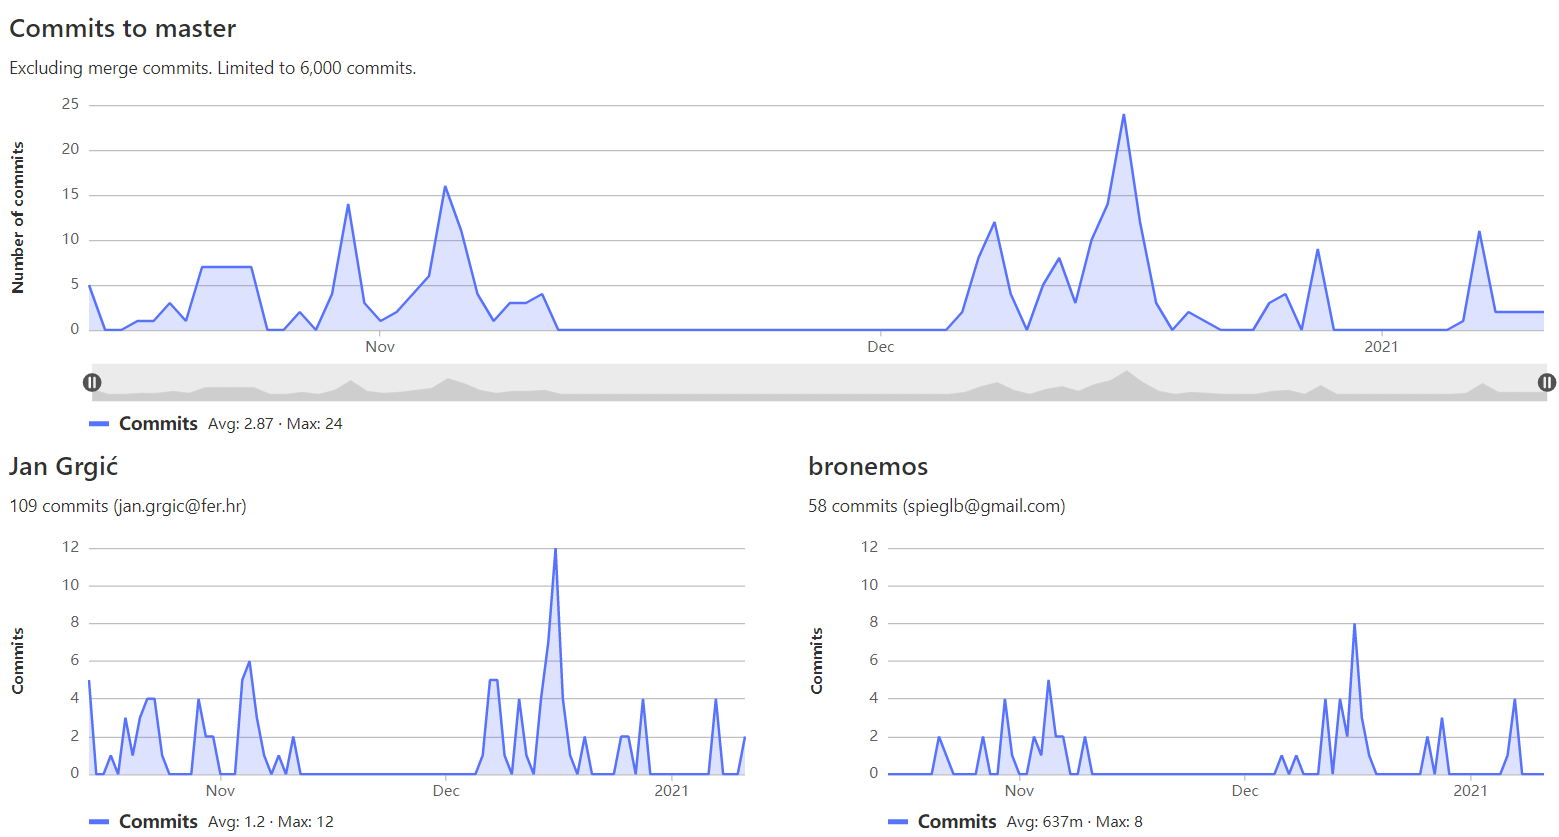
\includegraphics[scale=0.5]{slike/contributors.PNG}
	\caption{Contributors}
	\label{fig:promjene}
\end{figure}

\begin{figure}[H]
	\centering
	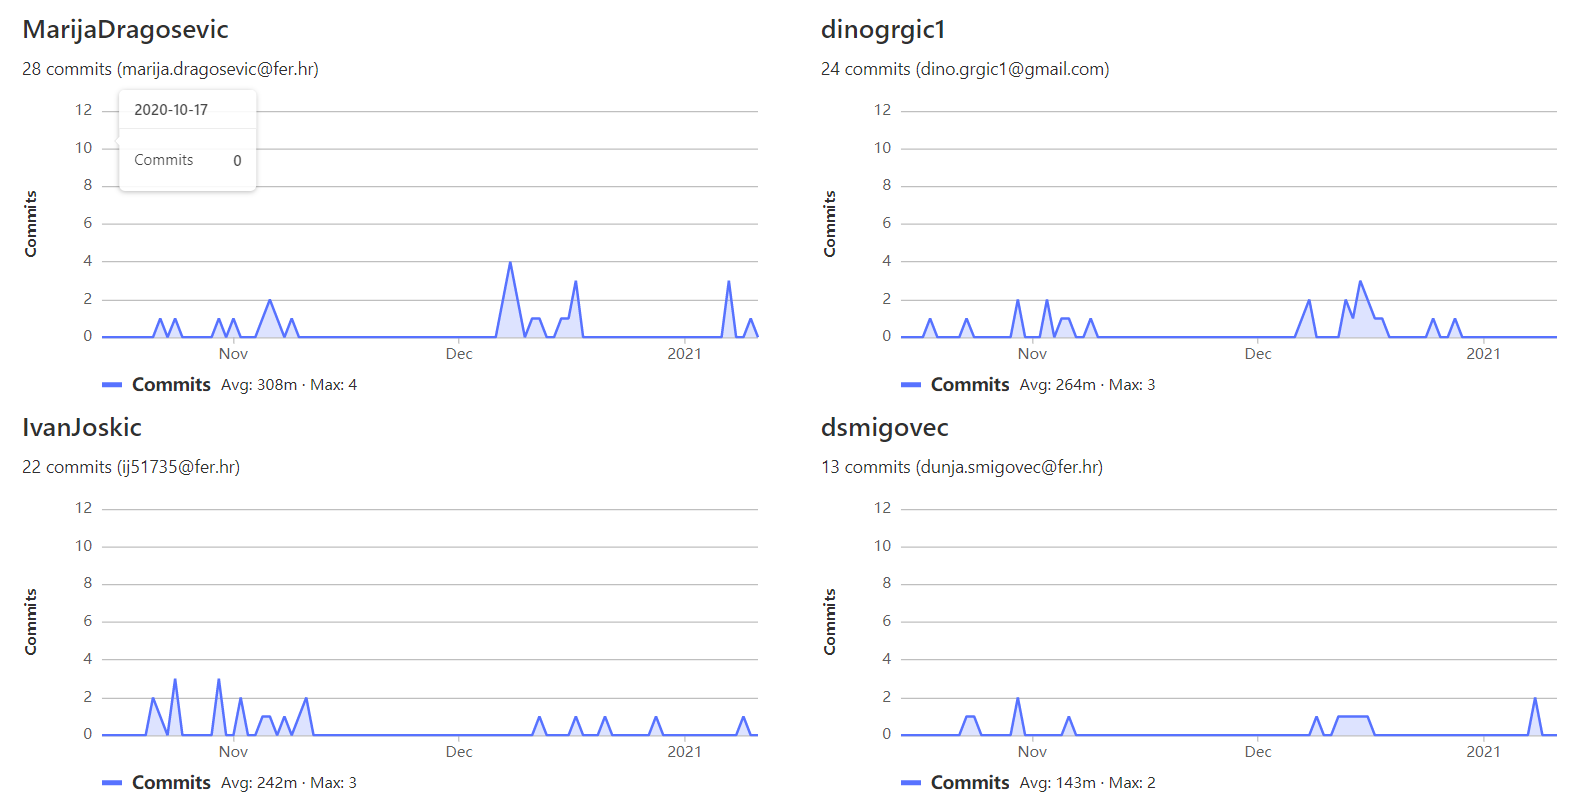
\includegraphics[scale=0.5]{slike/contributors1.PNG}
	\caption{Contributors}
	\label{fig:promjene}
\end{figure}

\begin{figure}[H]
	\centering
	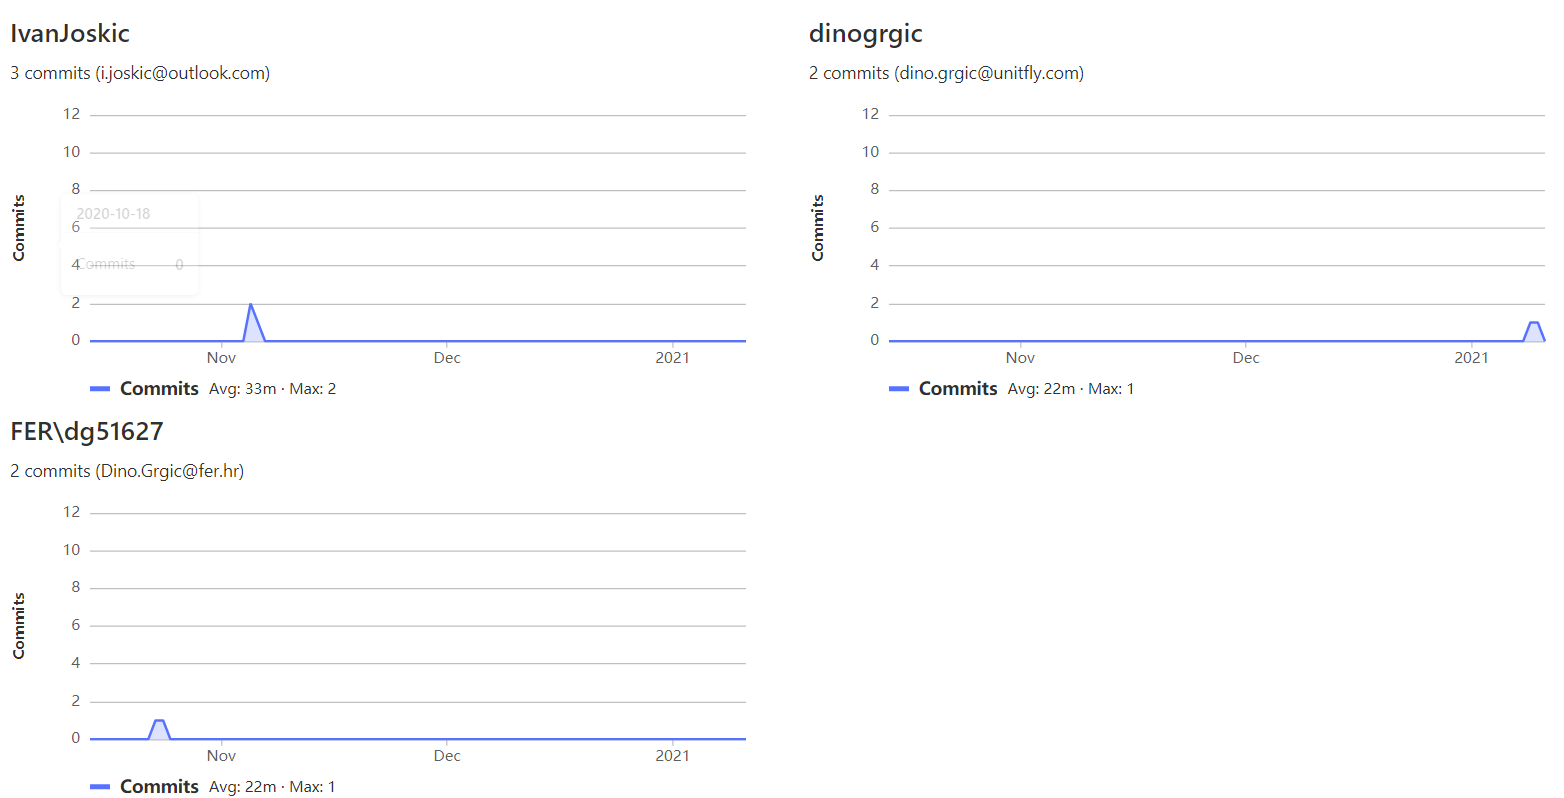
\includegraphics[scale=0.5]{slike/contributors2.PNG}
	\caption{Contributors}
	\label{fig:promjene}
\end{figure}


